% Equivalent of enabling ``-Wall -Wextra'' -- extra compile warnings.
\RequirePackage[l2tabu, orthodox]{nag}

\documentclass[capstoc,capschap,draftcls]{rpisudiss}
%\documentclass[draftcls]{rpisudiss}
\usepackage[utf8]{inputenc} % set input encoding (not needed with XeLaTeX)

% Latin Modern fonts - improved substitute for computer modern
% \usepackage{lmodern}

% Mathpazo - Palatino-matching math font.
\usepackage{mathpazo}

% TeX Gyre Pagella - version of Palatino
\usepackage{tgpagella}

% Improves type appearance through subtle changes.
\usepackage{microtype}

% Promises non-lousy copyright symbol.
\usepackage{textcomp}

% Super-common: support the \includegraphics command and options
\usepackage{graphicx}

% Add the \url command.
\usepackage{url}

% Supports cross-references to labels of form format:name (like fig:mypicture) and formats them nicer
% (Figure X) when you use \prettyref{fig:mypicture} instead of \ref{fig:mypicture}
\usepackage{prettyref}

% Font mappings for math stuff - makes better copy and paste.
\RequirePackage{cmap} % Works with multiple fonts, apparently.
%\RequirePackage{mmap} % Only compatible with computer modern math fonts.

% Make copy-pasteable PDF files.  Yes, it needs to be "input", not "usepackage"
\usepackage{ifxetex}
\ifxetex\else
  \input{glyphtounicode}
  \pdfgentounicode=1
\fi

%\usepackage[a-1b]{pdfx}

\widowpenalty=450                         % three times normal widow penalty
\clubpenalty=450                          % three times normal orphan penalty


%%% END Article customizations

%%% The "real" document content comes below...


\title{This is the title}
\author{Ryan Andrew Pavlik}

\isudegree{phd}
\isugradyear{2015}
\isusubmissiontype{dissertation}
\isumajor{Computer Science}
\isumajor{Human--Computer Interaction}
%\isumajors{Human--Computer Interaction, Computer Science}

\isuprofessor*{Judy M. Vance}% major prof
\isuprofessor*{Leslie Miller}% major prof
\isuprofessor{Debra Satterfield}
\isuprofessor{Jonathan Kelly}
\isuprofessor{David Weiss}
\isuprofessor{Horea Ilies}

% Some extra text to add to the draft footer each page if we're in draftcls mode.
\extradraftfooter{\textbf{Do not redistribute.}}

\begin{document}

\frontmatter
\maketitle

\tableofcontents
\listoffigures
\listoftables
\begin{abstract}
 Requirements for abstract:
 ``Formal citations, images, and complex equations should not be included in the Abstract.
 The text of the Abstract should not exceed 350 words.''
 This is a quote from \url{http://www.grad-college.iastate.edu/current/thesis/organizing_thesis/abstract.php} on 2014-07-11.
\end{abstract}

\chapter{Acknowledgements}
asdfawafesd

\mainmatter % Start the body of your doc with numbered chapters, etc.

\chapter{Intro}


A wide variety of software frameworks for building virtual reality
applications have been developed. The CAVE~Library initially developed
for use with the CAVE~Automated~Virtual~Environment \cite{Cruz-Neira1993}
is an example of early work in the systems category of virtual reality
frameworks. It has evolved into a commercial solution integrating
clustering support and focusing on multi-screen application development.
VR~Juggler introduced a highly modular architecture for VR applications
to provide a ``virtual platform'' for development and execution
on diverse systems \cite{Bierbaum2001,Bierbaum2005}.

frameworks. It has evolved into a commercial solution integrating
clustering support and focusing on multi-screen application development.
VR~Juggler introduced a highly modular architecture for VR applications

\[e=m\mathrm{c}^2\]

\section{Bla bla}
Later development
extended its use from high-end graphics systems to commodity computer
clusters \cite{Allard2002,Bierbaum2005}.


frameworks. It has evolved into a commercial solution integrating
clustering support and focusing on multi-screen application development.
VR~Juggler introduced a highly modular architecture for VR applications

\subsection{bla bla bla}
The commercial
VR authoring environment Virtools%
\footnote{\url{http://www.virtools.com/}%
} integrates a custom scripting language, VSL, for content creation.

frameworks. It has evolved into a commercial solution integrating
clustering support and focusing on multi-screen application development.
VR~Juggler introduced a highly modular architecture for VR applications
\chapter{middle}

A VR~JuggLua application uses both the osgLua module
and the VR~Juggler bindings included in the VR~JuggLua framework
to access a complete set of virtual reality functionality from Lua
(Figure \ref{fig:System-diagram}).
\begin{figure}
    \centering
    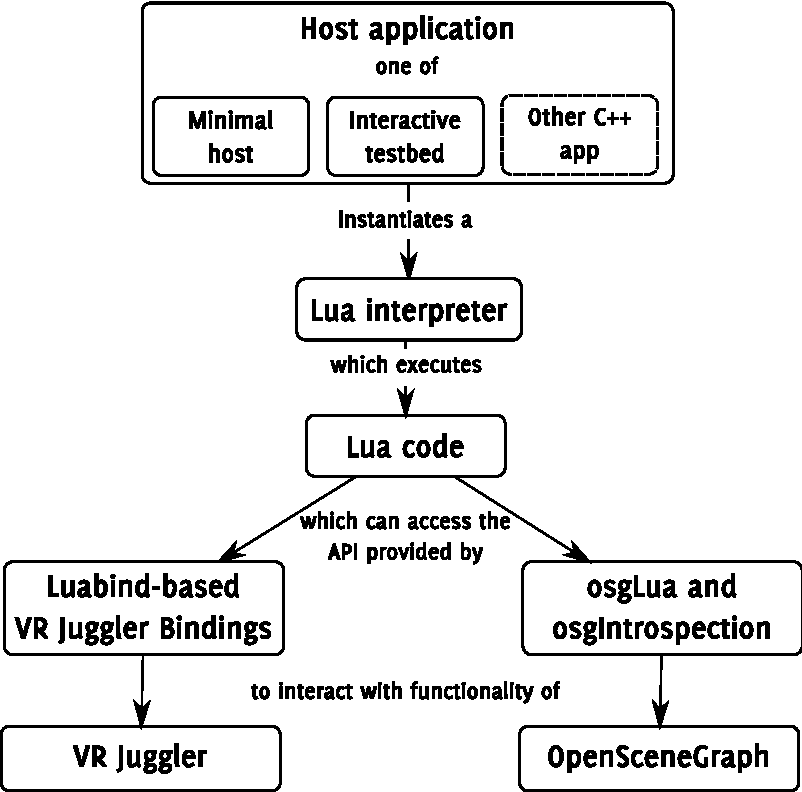
\includegraphics[width=1\columnwidth]{accessdiagram}
    \caption{\label{fig:System-diagram}System diagram}
\end{figure}


\chapter{Conclusion}

aefawefwaefadfwdcw


\bibliographystyle{abbrv}
\bibliography{vrjugglua}

\end{document}
